% Für Bindekorrektur als optionales Argument "BCORfaktormitmaßeinheit", dann
% sieht auch Option "twoside" vernünftig aus
% Näheres zu "scrartcl" bzw. "scrreprt" und "scrbook" siehe KOMA-Skript Doku
\documentclass[12pt,a4paper,titlepage,headinclude,bibtotoc]{scrartcl}


%---- Allgemeine Layout Einstellungen ------------------------------------------

% Für Kopf und Fußzeilen, siehe auch KOMA-Skript Doku
\usepackage[komastyle]{scrpage2}
\pagestyle{scrheadings}
\setheadsepline{0.5pt}[\color{black}]
\automark[section]{chapter}


%Einstellungen für Figuren- und Tabellenbeschriftungen
\setkomafont{captionlabel}{\sffamily\bfseries}
\setcapindent{0em}


%---- Weitere Pakete -----------------------------------------------------------
% Die Pakete sind alle in der TeX Live Distribution enthalten. Wichtige Adressen
% www.ctan.org, www.dante.de

% Sprachunterstützung
\usepackage[ngerman]{babel}

% Benutzung von Umlauten direkt im Text
% entweder "latin1" oder "utf8"
\usepackage[utf8]{inputenc}

% Pakete mit Mathesymbolen und zur Beseitigung von Schwächen der Mathe-Umgebung
\usepackage{latexsym,exscale,stmaryrd,amssymb,amsmath}

% Weitere Symbole
\usepackage[nointegrals]{wasysym}
\usepackage{eurosym}

% Anderes Literaturverzeichnisformat
%\usepackage[square,sort&compress]{natbib}

% Für Farbe
\usepackage{color}

% Zur Graphikausgabe
%Beipiel: \includegraphics[width=\textwidth]{grafik.png}
\usepackage{graphicx}

% Text umfließt Graphiken und Tabellen
% Beispiel:
% \begin{wrapfigure}[Zeilenanzahl]{"l" oder "r"}{breite}
%   \centering
%   \includegraphics[width=...]{grafik}
%   \caption{Beschriftung} 
%   \label{fig:grafik}
% \end{wrapfigure}
\usepackage{wrapfig}

% Mehrere Abbildungen nebeneinander
% Beispiel:
% \begin{figure}[htb]
%   \centering
%   \subfigure[Beschriftung 1\label{fig:label1}]
%   {\includegraphics[width=0.49\textwidth]{grafik1}}
%   \hfill
%   \subfigure[Beschriftung 2\label{fig:label2}]
%   {\includegraphics[width=0.49\textwidth]{grafik2}}
%   \caption{Beschriftung allgemein}
%   \label{fig:label-gesamt}
% \end{figure}
\usepackage{subfigure}

% Caption neben Abbildung
% Beispiel:
% \sidecaptionvpos{figure}{"c" oder "t" oder "b"}
% \begin{SCfigure}[rel. Breite (normalerweise = 1)][hbt]
%   \centering
%   \includegraphics[width=0.5\textwidth]{grafik.png}
%   \caption{Beschreibung}
%   \label{fig:}
% \end{SCfigure}
\usepackage{sidecap}

% Befehl für "Entspricht"-Zeichen
\newcommand{\corresponds}{\ensuremath{\mathrel{\widehat{=}}}}
% Befehl für Errorfunction
\newcommand{\erf}[1]{\text{ erf}\ensuremath{\left( #1 \right)}}

%Fußnoten zwingend auf diese Seite setzen
\interfootnotelinepenalty=1000

%Für chemische Formeln (von www.dante.de)
%% Anpassung an LaTeX(2e) von Bernd Raichle
\makeatletter
\DeclareRobustCommand{\chemical}[1]{%
  {\(\m@th
   \edef\resetfontdimens{\noexpand\)%
       \fontdimen16\textfont2=\the\fontdimen16\textfont2
       \fontdimen17\textfont2=\the\fontdimen17\textfont2\relax}%
   \fontdimen16\textfont2=2.7pt \fontdimen17\textfont2=2.7pt
   \mathrm{#1}%
   \resetfontdimens}}
\makeatother

%Honecker-Kasten mit $$\shadowbox{$xxxx$}$$
\usepackage{fancybox}

%SI-Package
\usepackage{siunitx}

%keine Einrückung, wenn Latex doppelte Leerzeile
\parindent0pt

%Bibliography \bibliography{literatur} und \cite{gerthsen}
%\usepackage{cite}
\usepackage{babelbib}
\selectbiblanguage{ngerman}

\begin{document}

\begin{titlepage}
\centering
\textsc{\Large Vermittlung strömungsphysikalischer Vorgänge im Experiment,
\\[1.5ex] Universität Göttingen}

\vspace*{3cm}

\rule{\textwidth}{1pt}\\[0.5cm]
{\huge \bfseries
  Versuch GPS  \\[1.5ex]
  Protokoll}\\[0.5cm]
\rule{\textwidth}{1pt}

\vspace*{3cm}

\begin{Large}
\begin{tabular}{ll}
Praktikant: &  Michael Lohmann\\
% &  Felix Kurtz\\
% &  Kevin Lüdemann\\
% &  Skrollan Detzler\\
 E-Mail: & m.lohmann@stud.uni-goettingen.de\\
% &  felix.kurtz@stud.uni-goettingen.de\\
% &  kevin.luedemann@stud.uni-goettingen.de\\
 Betreuer: & \\
 Versuchsdatum: & 07.12.2015\\
\end{tabular}
\end{Large}

\vspace*{0.8cm}

\begin{Large}
\fbox{
  \begin{minipage}[t][2.5cm][t]{6cm} 
    Testat:
  \end{minipage}
}
\end{Large}

\end{titlepage}

\tableofcontents

\newpage

\section{Einleitung}
\label{sec:einleitung}
Die Positionsbestimmung auf der Erde ist essentiell für weite Reisen.
Daher haben schon die Ägypter mit relativ einfachen Mitteln den Umfang der Erde bestimmt.
Heutzutage wird meist mit GPS-Satelliten navigiert.

\section{"`Fuß-GPS"'}
Das Funktionsprinzip von GPS kann man durch ein einfaches Experiment nachstellen:
Wenn drei Leute von bekannten Positonen aus zu einer vierten Person laufen, deren Ort unbekannt ist.
Die drei "`Photonen"' stoppen ihre Zeit, die sie benötigen, um zu der zu bestimmenden Stelle zu kommen.
Kennt man nun ihre ungefähre Geschwindigkeit und die Zeit, die sie um dem Start- zum Zielpunkt gebraucht haben, so kann man um den Startpunkt der einzelnen Personen Kreise ziehen.
Im Idealfall sollten sich alle drei Kreise an einem einzigen Punkt schneiden, welcher dann der Zielposition entspricht.
In der Realität wird dies nie erreicht werden, da die Personen nicht eine konstante Geschwindigkeit bei der Messung und bei der Geschwindigkeisbestimmung einhalten werden.

Übertragen auf das tatsächliche GPS bedeutet es, dass die Photonen sich zum Beispiel durch schwankende Ionosphären sich auch nicht konstant mit Lichtgeschwindigkeit fortbewegen.
Auch Streuung der Strahlung an der Umgebung kann zu störenden Einflüssen führen.
Die größte Unsicherheit besteht jedoch darin, dass das Empfangsgerät in der Regel keine Atomuhr hat, und so keine präzise Zeit messen kann.
Daher benötigt man nicht nur drei, sondern mindestens einen vierten Satelliten zur Positionsbestimmung.
Es gibt zwei Punkte, an denen sich der Empfänger befinden könnte, allerdings liegt der eine weit im Weltraum, so dass die Position auf der Erde doch wieder eindeutig ist.

Die Ergebnisse von unserem Versuch lassen sich auf dem Bild \ref{fig:gps} erkennen.
Dabei fällt auf, dass augenscheinlich alle Läufer bei der Messung zur Bestimmung der Geschwindigkeit etwas langsamer gegangen sind, als bei der tatsächlichen Messung.
Die tatsächliche Position der Zielperson liegt tatsächlich relativ genau zwischen den Kreisen.

\begin{figure}[h]
	\centering
	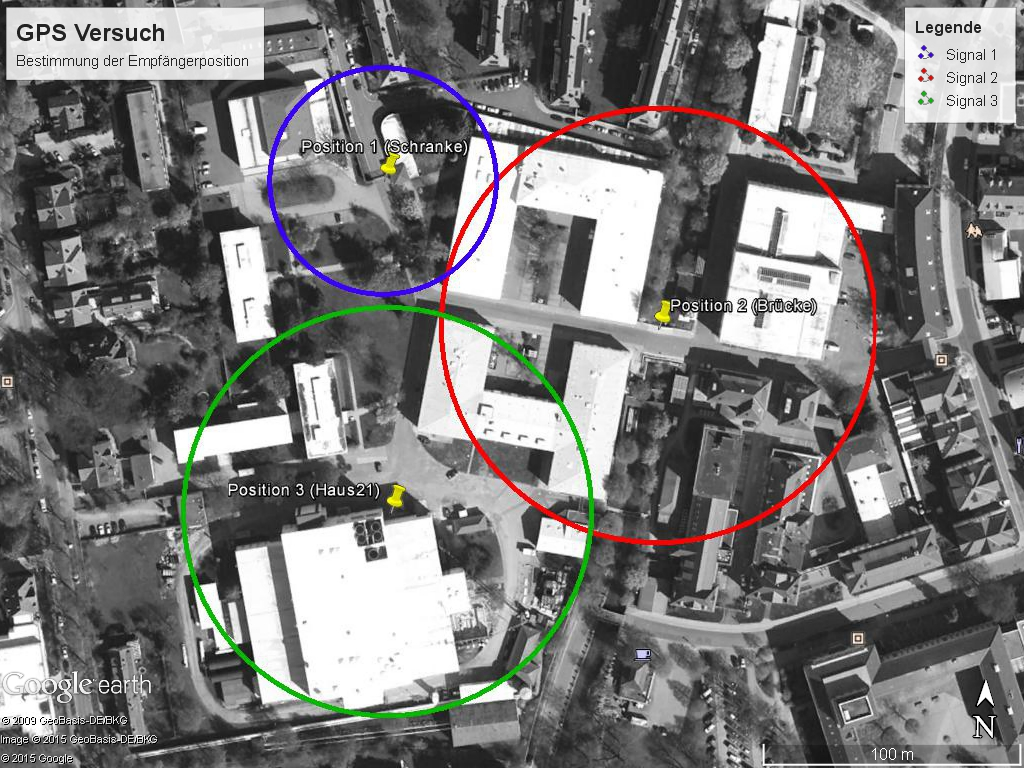
\includegraphics[scale=0.5]{GPS}
	\caption{Auftragung der Startpositionen der "`Photonen"', sowie der Entfernung, die sie jeweils zurückgelegt haben.}
	\label{fig:gps}
\end{figure}

\section{Bestimmung des Erdumfangs}
Schon die *****************************  maß vor über 3000 Jahren ********************************************************
den Umfang der Erde, als er bemerkte, dass genau zur Sonnenwende in *************************
ein Brunnen keinen Schatten im inneren hatte.
Zur selben Zeit jedoch in Alexandria (ca. 700km nördlicher gelegen) warf ein Turm einen Schatten.
Wäre die Erde eine Scheibe, so wäre dies nicht möglich bei dem riesigen Abstand, den die Sonne zur Erde hat.
Er bestimmte nun die Entfernung mit Hilfe eines Sklaventrupps, der die Strecke abging und durch Lederriemen in der Schrittlänge begrenzt war.
Dadurch konnte die Entfernung in Längeneinheiten dieser Schritte angegeben werden.
Da jedoch nicht die Luftlinie interessant war und auch diese durch Hindernisse nicht direkt zu bestimmen war, mussten die Sklaven immer genau in Nord-Süd-Richtung oder Ost-West-Richtung laufen.

Aus Höhe des Turms und Länge des Schattens ließ sich ein Winkel berechnen, der, wie in Abb. \ref{fig:umfang} zu sehen, so auch im Erdinneren zwischen den Orten vorhanden ist.










\bibliography{literatur}
\bibliographystyle{babalpha}
\end{document}
